\begin{ExerciseList}
  \setcounter{Exercise}{0}
%% \begin{figure}[H]
%%   \centering
%%   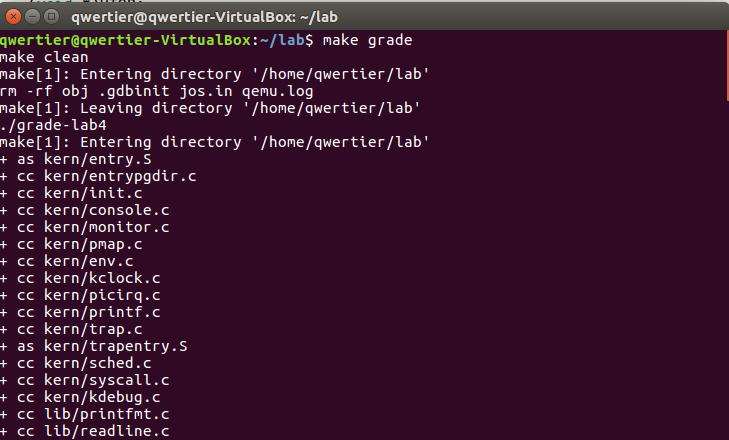
\includegraphics[width=6in]{figures/lab4/finish1.png}
%%   \caption{Lab4完成图}\label{fig:lab4:finish1}
  %% \end{figure}
  \section{Lab 2: Memory Management}

  \subsection{实验目的}

  操作系统必须要追踪记录哪些内存区域是空闲的,哪些是被占用的。JOS内核是以页(page)为最小粒度来管理内存的,它使用MMU来映射,保护每一块被分配出去的内存。在这里你要具体编写一下物理内存页的分配子函数。它利用一个结构体PageInfo的链表来记录哪些页是空闲的,链表中每一个结点对应一个物理页。

  \subsection{实验内容}

  \Exercise{在文件 kern/pmap.c 中,你必须要完成以下几个子函数的代码boot\_alloc(); mem\_init();  page\_init();  page\_alloc();page\_free();}

  先来看mem\_init()的代码。

  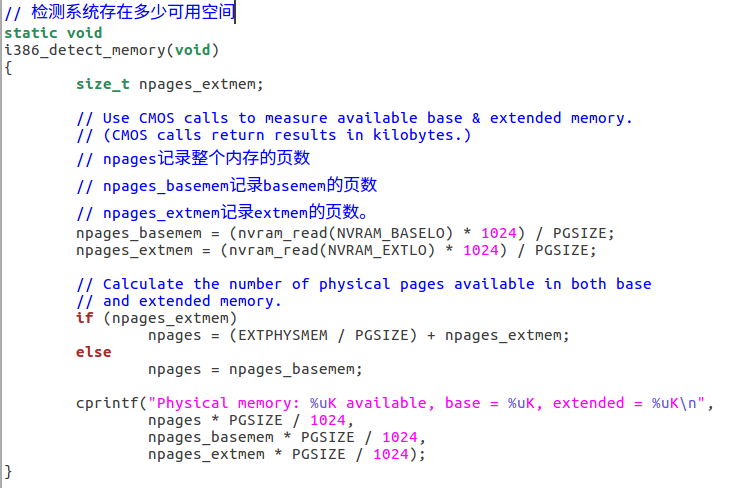
\includegraphics[width=6in]{figures/lab2/image40.png}

  这是i386\_detect\_memory 子函数的代码及注释。

  下面到了第一个需要添加的部分。

  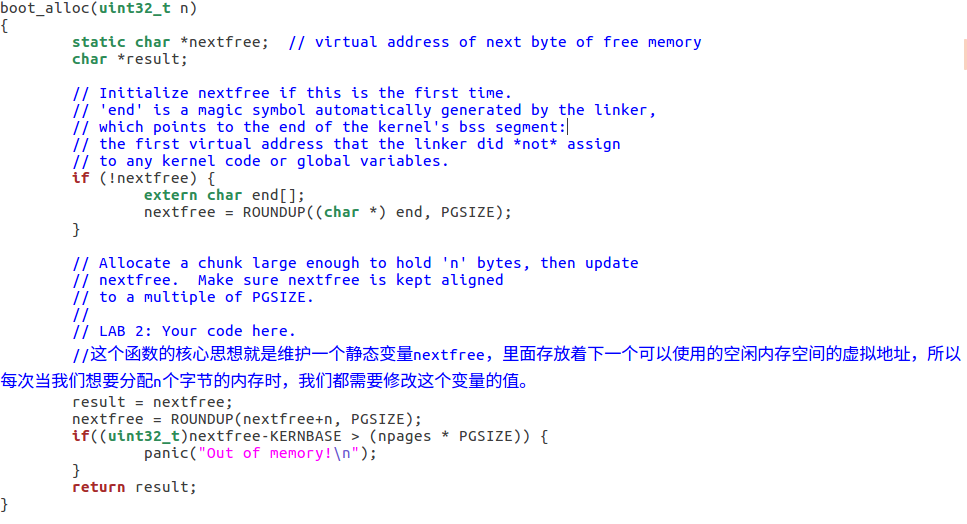
\includegraphics[width=6in]{figures/lab2/image41.png}

  Page\_init()需要补全的第二个函数。

  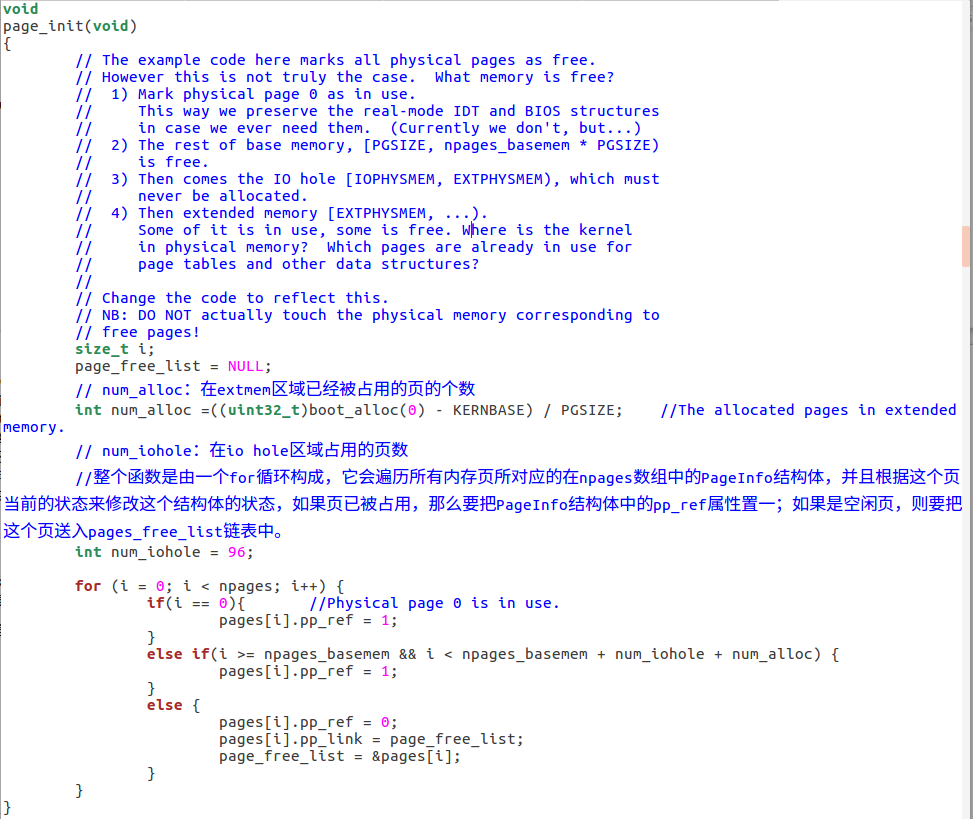
\includegraphics[width=6in]{figures/lab2/image42.png}

  接下来就是page\_alloc() 和page\_free()两个函数。

  先实现page\_alloc()函数,通过注释我们可以知道这个函数的功能就是分配一个物理页。而函数的返回值就是这个物理页所对应的PageInfo结构体。

  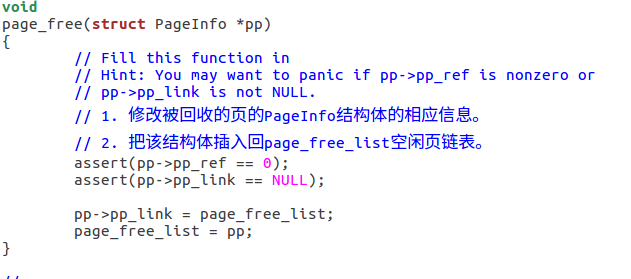
\includegraphics[width=6in]{figures/lab2/image44.png}

  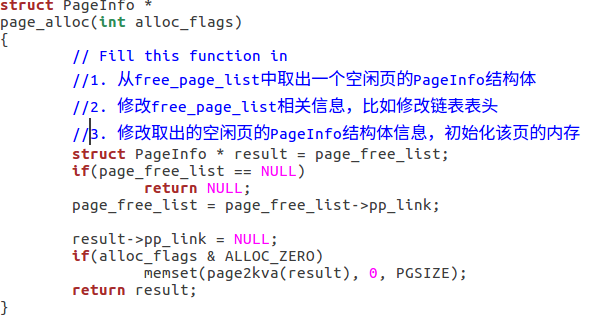
\includegraphics[width=6in]{figures/lab2/image43.png}

  实现page\_free()方法,根据注释可知,这个方法的功能就是把一个页的PageInfo结构体再返回给page\_free\_list空闲页链表,代表回收了这个页。

  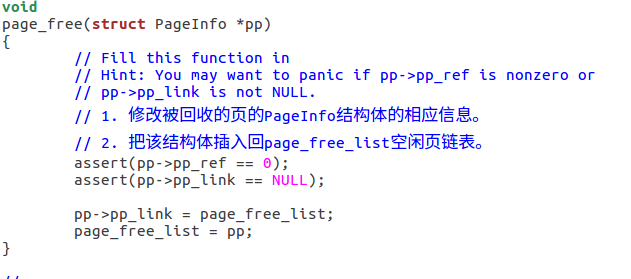
\includegraphics[width=6in]{figures/lab2/image44.png}

  一个虚拟地址(Virtual Address)是由两部分组成,一个是段选择子(segment selector),另一个是段内偏移(segment offset)。一个线性地址(Linear Address)指的是通过段地址转换机构把虚拟地址进行转换之后得到的地址。一个物理地址(Physical Addresses)是分页地址转换机构把线性地址进行转换之后得到的真实的内存地址,这个地址将会最终送到你的内存芯片的地址总线上。

  xp/Nx paddr – 查看paddr物理地址处开始的,N个字的16进制的表示结果。

  info registers – 展示所有内部寄存器的状态。

  info mem – 展示所有已经被页表映射的虚拟地址空间,以及它们的访问优先级。

  info pg – 展示当前页表的结构。

  \Exercise{参阅“ 英特尔80386参考手册”的第5章和第6章 ,如果还没有这样做的话。仔细阅读关于页面翻译和页面保护的章节(5.2和6.4)。浏览有关细分的部分; 而JOS使用分页硬件进行虚拟内存和保护时,在x86上不能禁用段转换和基于段的保护,因此需要对其进行基本的了解。}

  \Exercise{了解QEMU的一些指令,查看内存。}

  \Exercise{完成pgdir\_walk()boot\_map\_region()page\_lookup()   page\_remove()page\_insert()}

  函数给定一个页目录表指针 pgdir ,该函数应该返回线性地址va所对应的页表项指针。

  代码截图如下:


  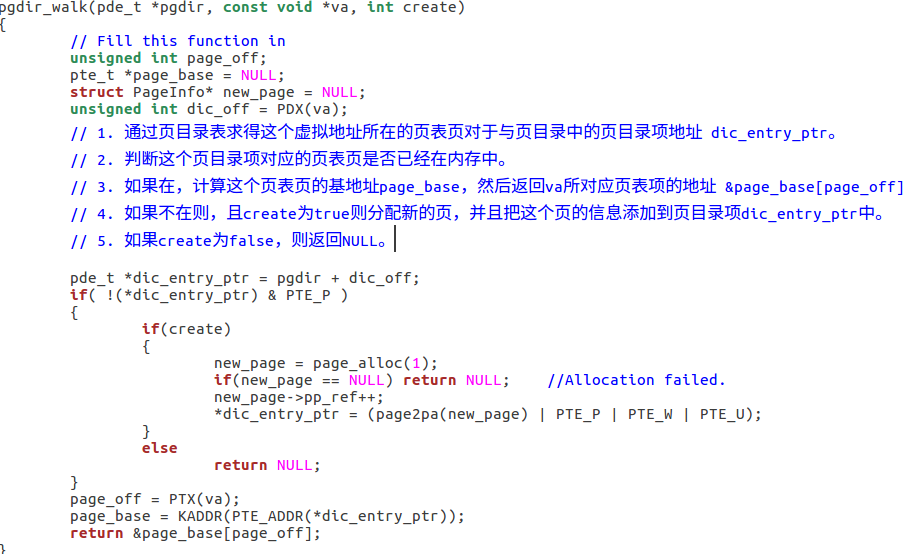
\includegraphics[width=6in]{figures/lab2/image45.png}


  boot\_map\_region函数,把虚拟地址空间范围[va, va+size)映射到物理空间[pa, pa+size)的映射关系加入到页表pgdir中。这个函数主要的目的是为了设置虚拟地址UTOP之上的地址范围,这一部分的地址映射是静态的,在操作系统的运行过程中不会改变,所以这个页的PageInfo结构体中的pp\_ref域的值不会发生改变。


      代码截图:


      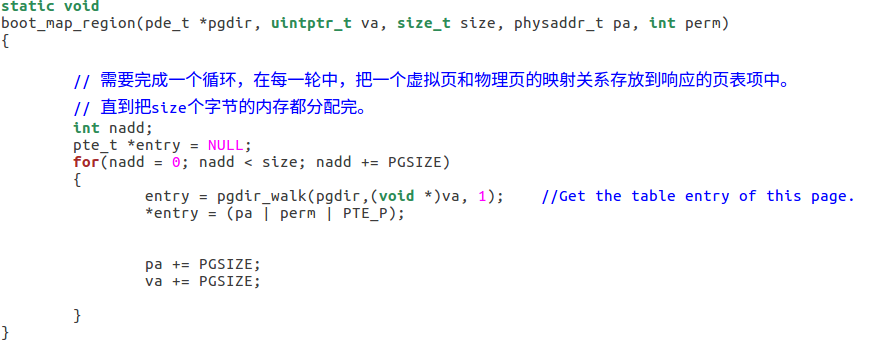
\includegraphics[width=6in]{figures/lab2/image46.png}


      page\_insert()功能上是完成:把一个物理内存中页pp与虚拟地址va建立映射关系。


      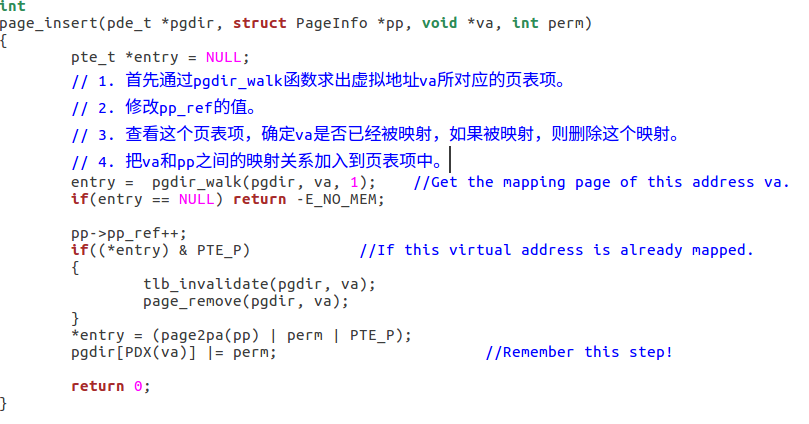
\includegraphics[width=6in]{figures/lab2/image47.png}

      pp->pp\_ref++这条语句,一定要放在page\_remove之前。

      接下来继续完成page\_lookup()函数,返回虚拟地址va所映射的物理页的PageInfo结构体的指针,如果pte\_store参数不为0,则把这个物理页的页表项地址存放在pte\_store中。


      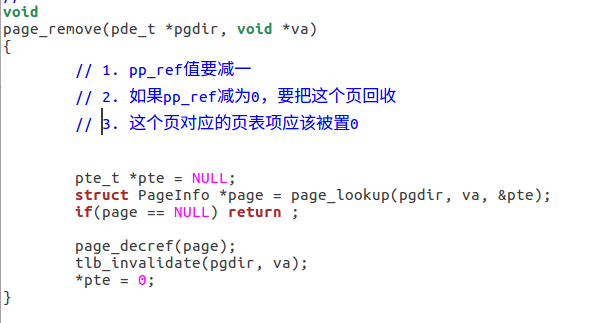
\includegraphics[width=6in]{figures/lab2/image48.png}

      page\_remove函数,功能就是把虚拟地址va和物理页的映射关系删除。

      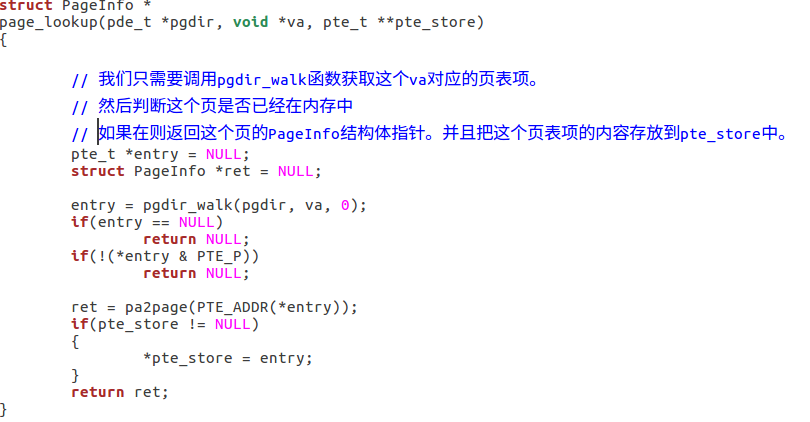
\includegraphics[width=6in]{figures/lab2/image49.png}

  由于内核和用户进程只能访问各自的地址空间,所以我们必须在x86页表中使用访问权限位(Permission Bits)来使用户进程的代码只能访问用户地址空间,而不是内核地址空间。否则用户代码中的一些错误可能会覆写内核中的数据,最终导致内核的崩溃。处在用户地址空间中的代码不能访问高于ULIM的地址空间,但是内核可以读写这部分空间。而内核和用户对于地址范围[UTOP, ULIM]有着相同的访问权限,那就是可以读取但是不可以写入。这一个部分的地址空间通常被用于把一些只读的内核数据结构暴露给用户地址空间的代码。在UTOP之下的地址范围是给用户进程使用的,用户进程可以访问,修改这部分地址空间的内容。

  \Exercise{剩下的工作就是要完善mem\_init()函数,现在要完善的功能就是把关于操作系统的一些重要的地址范围映射到现在的新页目录项上kern\_pgdir上。这里我们可以利用前面定义过的boot\_map\_region函数。}






\end{ExerciseList}
